\documentclass{article}
% translate with >> pdflatex -shell-escape <file>

% This file is used as unit test for pgfplots, copyright by Christian Feuersaenger.
% 
% See
%   http://pgfplots.sourceforge.net/pgfplots.pdf
% for pgfplots.
%
% Any required input files (for <plot table> or <plot file> or the table package) can be downloaded
% at
% http://www.ctan.org/tex-archive/graphics/pgf/contrib/pgfplots/doc/latex/
% and
% http://www.ctan.org/tex-archive/graphics/pgf/contrib/pgfplots/doc/latex/plotdata/

\usepackage{pgfplots}
\pgfplotsset{compat=newest}

\pagestyle{empty}

\begin{document}

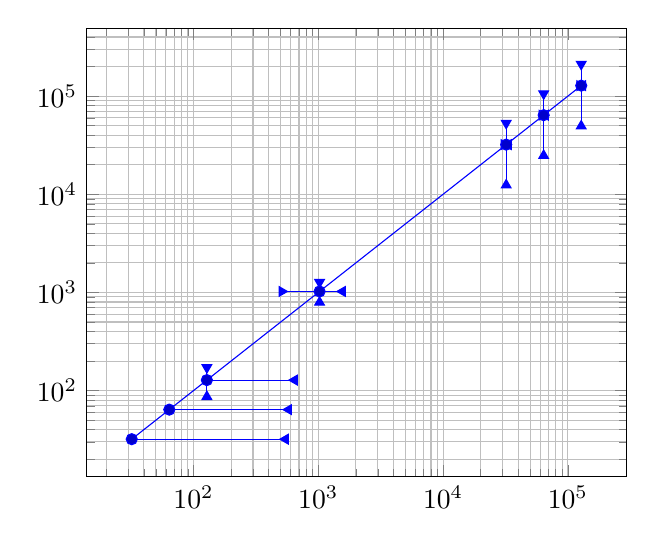
\begin{tikzpicture}
\begin{loglogaxis}[
	grid=both]
\addplot plot[
	error bars/.cd,
	y dir=both,y explicit relative,
	x dir=both,x fixed=500,
	error mark=triangle*,
]
	coordinates {
		(32,32)
		(64,64)
		(128,128) +- (0,0.3)
		(1024,1024) +- (0,0.2)
		(32068,32068)  +- (0,0.6)
		(64000,64000) +- (0,0.6)
		(128000,128000) +- (0,0.6)
	};

\end{loglogaxis}
\end{tikzpicture}
\end{document}
